%%%%%%%%%%%%%%%%%%%%%%%%%%%%%%%%%%%%%%%%%%%%%%%%%%%%%
%			ŠABLONA PÍSNIČEK v. 18.09               %
%%%%%%%%%%%%%%%%%%%%%%%%%%%%%%%%%%%%%%%%%%%%%%%%%%%%%
% Tento soubor slouží jako (naučná) šablona, pomocí 
% které lze vytvářet zdrojové soubory k jednotlivým 
% písním.
%%%%%%%%%%%%%%%%%%%%%%%%%%%%%%%%%%%%%%%%%%%%%%%%%%%%%
%			Jak psát soubory songů?                 %
%%%%%%%%%%%%%%%%%%%%%%%%%%%%%%%%%%%%%%%%%%%%%%%%%%%%%
%	1. Text písně se začíná psát na místě START 
%	   a končí na místě END. Zbylý text ignorujte.
%	2. Jak bude vypadat pdf písně zjistíte po tom, 
%	   co soubor zkompilujete pomocí souboru   
%      ../Generator/generator. 
%	3. Při psaní dodržujte následující TeX pravidla:
%	 a) Nový řádek napíšete pomocí dvou odsazení 
%	    tedy dvou enterů.
%	 b) Nová sloka se píší pomocí \sloka a odsazení.
%		Refrén se píše jako \refren, v případě více 
%		refrénů \refren[č. refrénu].
%	 c) Akordy se píšou tak, že napíšete před slovo,
%	    kde chcete mít akord (bez mezery):
%		^{AKORD1\,AKORD2...}.
%	4. Pokud chcete ušetřit tvůrcům práci, tak 
%	   si přečtěte další poučný soubor o typografii 
%	   ../../Typo_pravidla.txt.
%	5. Akordy stačí psát jen do první sloky, když 
%	   se nezmění -- kytaristé to zvládnou
%	7. Název písně pište na místo [NÁZEV] a autora 
%	   pište na místo [AUTOR] 
%	7. Jak psát věci na české klávesnici:
%	   \ = alt gr + q; [/] = alt gr f/g; 
%      {/} = alt gr + b/n; ^ = alt gr + 3 , cokoliv
%%%%%%%%%%%%%%%%%%%%%%%%%%%%%%%%%%%%%%%%%%%%%%%%%%%%%
%			Jak kompilovat jednotlivé písně?        %
%%%%%%%%%%%%%%%%%%%%%%%%%%%%%%%%%%%%%%%%%%%%%%%%%%%%%
%	1. Více návodu je k tomuto napsáno v souboru 
%      ../Generator/generator. 
%%%%%%%%%%%%%%%%%%%%%%%%%%%%%%%%%%%%%%%%%%%%%%%%%%%%%
%			Jak kompilovat celý zpěvník?			%
%%%%%%%%%%%%%%%%%%%%%%%%%%%%%%%%%%%%%%%%%%%%%%%%%%%%%
%	1. Více návodu je k tomuto napsáno v souboru
%	   ../Cely_zpevnik/zpevnik.tex.
%%%%%%%%%%%%%%%%%%%%%%%%%%%%%%%%%%%%%%%%%%%%%%%%%%%%%
\begin{song}{title=\predtitle \centering Wonderwall \\\large Oasis }  %% sem se napíše jméno songu a autor

\vspace*{.5cm}

\begin{centerjustified}
\vetsi


\kapodastr{2}

\predehra
\textbf{$4\times$ Emi7 G Dsus4 A7sus4}


\sloka
^{Emi7\z}Today is ^{G\z}gonna be the day

That they're ^{Dsus4\z}gonna throw it back ^{A7sus4}to~you.

^{Emi7\z}By~now you ^{G\z}should've somehow

^{Dsus4}Realised what you ^{\z A7sus4}gotta~do.


^{Emi7}I~don't believe that ^{G\z}anybody

^{\z Dsus4}Feels the ^*{A7sus4}way~I~do~abo ut you ^{Cadd9}now. ^{Dsus4 A7sus4}


\sloka
^{Emi7 \z}Backbeat the ^{G \z}word is on the street

That the ^{Dsus4 \,}fire in your heart ^{A7sus4 \z}is~out.

^{Emi7 \z}I'm~sure you've ^{G \z}heard it all before

But you ^{Dsus4}never really had ^{A7sus4 \z}a~doubt.

^{Emi7 \z}I~don't believe that ^{G \z}anybody ^{Dsus4}feels

The way I ^{A7sus4 \z}do~about you ^{Emi7}now. ^{G Dsus4 A7sus4}


\end{centerjustified}
\newpage
\begin{centerjustified}


\refren[1]
And ^{Cadd9 \z}all~the roads ^{Dsus4}we~have~to walk ^*{Emi7}are~w inding

And ^{Cadd9 \z}all~the lights ^{\z Dsus4}that lead us there ^*{Emi7}are~bl inding

^{Cadd9}There are many ^*{Dsus4}thing s that I would

^*{G\z}Li ke to ^{D/F# \z}say~to ^{Emi7}you

But ^*{G \z}I~don 't know ^{\z A7sus4}how.~~~


\refren[2]
Because ^{Cadd9 \z}maybe ^{Emi7 G}

You're ^{Emi7 \z}gonna be the one that ^{Cadd9\z}saves me? ^{Emi7 G}

And ^{Emi7}after ^{Cadd9 \z}all~~~~~~ ^{Emi7 G}

You're ^{Emi7}my ^{\z Cadd7}wonderwall.~~~~ ^{Emi7 G Emi7(Break)}

\sloka
Today was gonna be the day

But they'll never throw it back to you.

By now you should've somehow

Realised what you're not to do.

I don't believe that anybody

Feels the way I do

About you ^{Cadd9}now.~ ^{Dsus4 A7sus4}


\refren[1]


\refren[2]
I said maybe \dots

\refren[2]
I said maybe (I said maybe) \dots

\phantom{.}

I said maybe. (I said maybe)

/: You're ^{Emi7}gonna be the one that ^{Cadd9\z}saves me? (that ^{Emi7 \z}saves ^{\z G}me) :/

You're gonna be the one that saves me? (that saves me)

\ssloka{\textbf{Sólo:}}\\
\centering
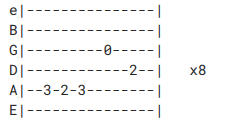
\includegraphics[scale=3]{../taby/wonderwall.png}

\vspace{.5cm}
% 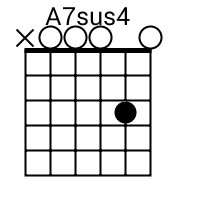
\includegraphics[width=3cm]{../Akordy/a7sus4.png} % akordy se tu hraji celkove jinak, tak ze se dohromady lepe prehmatavaji -> tzn toto by tu bylo matouci
\end{centerjustified}
\setcounter{Slokočet}{0}
\end{song}
